\documentclass[12pt]{article}

\usepackage[utf8]{inputenc}
\usepackage[T1]{fontenc}
\usepackage{lmodern}
\usepackage[spanish]{babel}
\usepackage{booktabs}
\usepackage{amsmath}
\usepackage{forest}
\usepackage{float}
\usepackage{listings}
\usepackage{xcolor}
\usepackage{tikz}
\usepackage{hyperref}

\definecolor{codegreen}{rgb}{0,0.6,0}
\definecolor{codegray}{rgb}{0.5,0.5,0.5}
\definecolor{codepurple}{rgb}{0.58,0,0.82}
\definecolor{backcolour}{rgb}{0.95,0.95,0.92}

\lstdefinestyle{mystyle}{
    backgroundcolor=\color{backcolour},   
    commentstyle=\color{codegreen},
    keywordstyle=\color{magenta},
    numberstyle=\tiny\color{codegray},
    stringstyle=\color{codepurple},
    basicstyle=\ttfamily\footnotesize,
    breakatwhitespace=false,         
    breaklines=true,                 
    captionpos=b,                    
    keepspaces=true,                 
    numbers=left,                    
    numbersep=5pt,                  
    showspaces=false,                
    showstringspaces=false,
    showtabs=false,                  
    tabsize=2
}

\lstset{style=mystyle}

\sloppy
\setlength{\parindent}{0pt}

\begin{document}

\begin{center}
  {\LARGE \textbf{Python para IO}}\\[0.5em]
  {Investigación Operativa, Universidad de San Andrés}
\end{center}

Si encuentran algún error en el documento o hay alguna duda, mandenmé un mail a rodriguezf@udesa.edu.ar y lo revisamos.

\section{Motivación}
Python es un lenguaje de programación versátil que nos va a permitir resolver problemas de optimización. El proceso típico va a ser:
\begin{enumerate}
    \item Identificar el problema
    \item Crear el modelo matemático
    \item Implementar y resolver usando Python
\end{enumerate}

En Investigación Operativa usamos Python porque los problemas con los que nos vamos a encontrar no son resolubles a mano. Necesitamos herramientas que nos permitan resolverlos de manera eficiente, y Python es una de las herramientas más fáciles de usar para resolver problemas de optimización.

\vspace{0.5cm}
\begin{tabular}{ccc}
    \textbf{Problema} & \hspace{0.8cm} $\rightarrow$ \hspace{0.8cm} \textbf{Modelado} \hspace{0.8cm} $\rightarrow$ \hspace{0.8cm} & \textbf{Optimización}
\end{tabular}

\begin{figure}[H]
    \centering
    \begin{tikzpicture}[node distance=2cm, auto, thick, scale=1.3, every node/.style={transform shape}]
        % Problema (izquierda)
        \foreach \i in {1,2,3} {
            \draw[fill=red!30] (-3,1.2-\i*0.8) circle (0.35) node {\i};
        }
        \foreach \i in {1,2,3,4} {
            \draw[fill=blue!20] (-2,1.5-\i*0.7) circle (0.32) node {\i};
        }
        % Conexiones
        \draw[thick, gray!70] (-3,0.4) -- (-2,0.8);
        \draw[thick, gray!70] (-3,0.4) -- (-2,0.1);
        \draw[thick, gray!70] (-3,0.4) -- (-2,-0.6);
        \draw[thick, gray!70] (-3,0.4) -- (-2,-1.3);
        \draw[thick, gray!70] (-3,-0.4) -- (-2,0.8);
        \draw[thick, gray!70] (-3,-0.4) -- (-2,0.1);
        \draw[thick, gray!70] (-3,-0.4) -- (-2,-0.6);
        \draw[thick, gray!70] (-3,-0.4) -- (-2,-1.3);
        \draw[thick, gray!70] (-3,-1.2) -- (-2,0.8);
        \draw[thick, gray!70] (-3,-1.2) -- (-2,0.1);
        \draw[thick, gray!70] (-3,-1.2) -- (-2,-0.6);
        \draw[thick, gray!70] (-3,-1.2) -- (-2,-1.3);
    \end{tikzpicture}
    \hfill
    \begin{tikzpicture}[node distance=2cm, auto, thick, scale=0.9, every node/.style={transform shape}]
        % Modelado (centro)
        \node[align=center] at (1.7,-0.2) {
            $Z = 3000x_1 + 5000x_2$\\[0.2em]
            $\begin{aligned}
            2x_2 &\leq 12\\
            3x_1 + 2x_2 &\leq 18\\
            x_1 &\geq 0 \\
            x_2 &\geq 0
            \end{aligned}$
        };
    \end{tikzpicture}
    \hfill
    \begin{tikzpicture}[node distance=2cm, auto, thick, scale=0.9, every node/.style={transform shape}]
        % Optimización (derecha)
        % Incluir imagen 3D
        \node[inner sep=0pt] at (5.5,1.2) {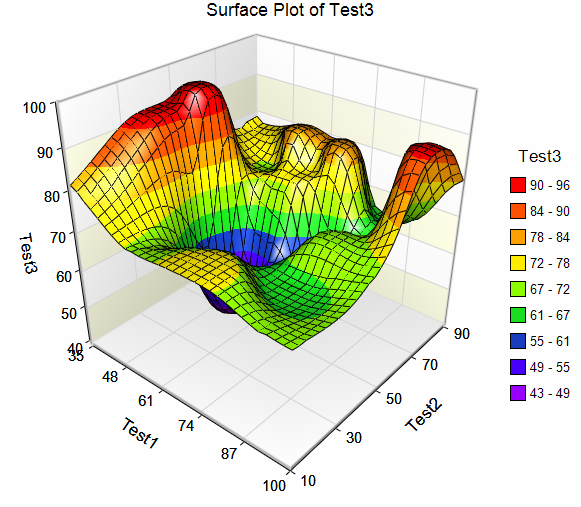
\includegraphics[width=5cm]{3d_graph.png}};
    \end{tikzpicture}
\end{figure}

\section{Conceptos Básicos de Python}
\subsection{Variables y Tipos de Datos}
En Python podemos asignar un objeto a una variable usando el signo =.

\begin{lstlisting}[language=Python]
texto = "Hello World"
numero = 5
numero_con_coma = 1.3
mi_lista = [1, 2, 3, 4]
mi_tupla = (1, 2, 4)
\end{lstlisting}

\subsection{Operaciones Matemáticas}
Las operaciones matemáticas básicas en Python son:
\begin{itemize}
    \item Suma: +
    \item Resta: -
    \item Multiplicación: *
    \item División: /
    \item División entera: //
    \item Potencia: **
    \item Resto: \%
\end{itemize}

\subsection{Print}
Para mostrar valores o resultados usamos la función print:

\begin{lstlisting}[language=Python]
a = 10
b = 20
print("El resultado es", a+b)
# Output:
# El resultado es 30
\end{lstlisting}

\subsection{Estructuras de Control}
\subsubsection{Condicionales (if/else)}
\begin{lstlisting}[language=Python]
if a == b:
    print("Son iguales")
else:
    print("Son distintos")
# Output:
# Son distintos
\end{lstlisting}

\subsubsection{Bucles}
El bucle for es muy útil para iterar sobre secuencias:
\begin{lstlisting}[language=Python]
for i in range(4):
    print(i)
# Output:
# 0
# 1
# 2
# 3
\end{lstlisting}

El bucle while se ejecuta mientras una condición sea verdadera:
\begin{lstlisting}[language=Python]
i = 0
while i < 4:
    print(i)
    i = i + 1
# Output:
# 0
# 1
# 2
# 3
\end{lstlisting}

\section{Librerías Principales}
Para nuestro trabajo en IO, usaremos principalmente:
\begin{itemize}
    \item \textbf{NumPy}: Para manipulación de matrices y vectores
    \item \textbf{Matplotlib}: Para visualización de datos
    \item \textbf{PICOS}: Para problemas de optimización
    \item \textbf{SciPy}: Para optimización no lineal
\end{itemize}

El estándar de importación que usaremos es:
\begin{lstlisting}[language=Python]
import numpy as np
import scipy as scp
import picos
import matplotlib.pyplot as plt
\end{lstlisting}

\section{NumPy}
NumPy es fundamental para trabajar con arrays y matrices:
\begin{lstlisting}[language=Python]
array = np.array([1, 2, 3, 4])

# Acceso a elementos
print(array[0])  # Primer elemento
# Output:
# 1

# Operaciones matriciales
matriz = np.array([[1, 2], [3, 4]])
print(matriz[0, 1])  # Elemento en fila 0, columna 1
# Output:
# 2
\end{lstlisting}

\section{Ejercicios Prácticos}
\subsection{Ejercicio 1: Listas y Promedios}
Vamos a resolver los siguientes puntos:
\begin{enumerate}
    \item Generar una lista L con todos los números pares hasta el 20
    \item Solo guardar los múltiplos de 4
    \item Calcular la media: $\langle L \rangle = \frac{\sum L_i}{N}$
\end{enumerate}

\begin{lstlisting}[language=Python]
L = []
for i in range(20):
    if i % 2 == 0:
        L.append(i)

L_filtrado = []
for i in L:
    if i % 4 == 0:
        L_filtrado.append(i)

media = np.mean(L_filtrado)
print(media)
# Output:
# 6.0
\end{lstlisting}

\subsection{Ejercicio 2: Función Múltiplos}
\begin{enumerate}
    \item Definir la función múltiplos que acepte como input el número hasta donde quiero obtener los números pares y el número del que quiero que sean múltiplos
    \item Graficar los puntos usando matplotlib
\end{enumerate}

\begin{lstlisting}[language=Python]
def multiplos(n, m):
    L = []
    for i in range(n):
        if i % m == 0:
            L.append(i)
    return L

plt.plot(multiplos(100, 4))
plt.show()
\end{lstlisting}

\begin{center}
\Huge\textbf{A programar se aprende programando.}
\end{center}

\end{document}